
\documentclass[runningheads]{llncs}

% to have bookmarks in pdf
% remove for final version
\usepackage[open,openlevel=5]{bookmark}
\setcounter{tocdepth}{5}

\usepackage{graphicx}
% Used for displaying a sample figure. If possible, figure files should
% be included in EPS format.
%

\graphicspath{{./images/}}

\usepackage{hyperref}
% If you use the hyperref package, please uncomment the following line
% to display URLs in blue roman font according to Springer's eBook style:
\renewcommand\UrlFont{\color{blue}\rmfamily}

%\usepackage{courier}
\usepackage{listings, color}
\hypersetup{
  colorlinks   = true,
  linkcolor  = blue,
  citecolor  = blue,
  urlcolor   = blue
}



%\usepackage{newtxtext}
%\usepackage{newtxmath}
\usepackage[zerostyle=b,scaled=.88]{newtxtt}

% nicer bold
\renewcommand{\bfdefault}{b}%


% make paragraph headings bold instead of italics
\renewcommand{\paragraph}{\textbf}%

\definecolor{dkgreen}{rgb}{0,0.6,0}
\definecolor{gray}{rgb}{0.5,0.5,0.5}
\definecolor{mauve}{rgb}{0.58,0,0.82}

\lstdefinestyle{scala}{
  language=scala,
  basicstyle=\footnotesize\ttfamily,
%  basicstyle=\scriptsize\ttfamily, % kai: temporary 
  breaklines=true,
  keywordstyle=\color{blue},
  commentstyle=\color{dkgreen},
  numbers=left,
  %frame=single, % Border around box
  %numbersep=-7pt,
  numberstyle=\color{gray},
  stringstyle=\color{mauve}
}

\lstdefinestyle{stainless}{
  numbers=none,
  breaklines=true,
  breakautoindent=true,
  breakindent=63pt,
  basicstyle=\footnotesize\ttfamily
}
 
\newcommand{\todo}[1]{{\par \color{red}#1}}


\begin{document}

\title{Towards Verifying the Bitcoin-S Library}

\author{Ramon Boss \and Kai Brünnler \and Anna Doukmak}

\authorrunning{R. Boss et al.}
\institute{Bern University of Applied Sciences, CH-2501 Biel, Switzerland
\email{ramon.boss@outlook.com, kai.bruennler@bfh.ch,\\anna.doukmak@gmail.com}}

\maketitle             

\begin{abstract}
  We try to verify properties of the bitcoin-s library, a Scala
  implementation of parts of the Bitcoin protocol. We use the
  Stainless verifier which supports programs in subset of Scala called
  the \emph{Pure Scala Fragment}. We first try to verify the property
  that regular transactions do not create new money. It turns out that
  there is too much code involved that lies outside of the supported
  fragment to make this feasible. However, in the process we uncover
  and fix a bug in bitcoin-s. We then turn to a much simpler (and less
  interesting) property: that adding zero satoshis to a given amount
  of satoshis yields the given amount of satoshis. Here as well a
  significant part of the relevant code lies outside of the supported
  fragment. However, after a series of equivalent transformations we
  arrive at code that we successfully verify.

\keywords{Bitcoin  \and Scala \and Bitcoin-S \and Stainless.}
\end{abstract}



\section{Introduction}

For software handling cryptocurrency, correctness is clearly crucial.
However, even in very well-tested software such as Bitcoin Core,
serious bugs occur. The most recent example is the bug found in
September 2018 \cite{cve201817144} which essentially allowed to
arbitrarily create new coins. Such software is thus a worthwhile
target for formal verification. In this work, we set out to verify
properties of the bitcoin-s library with the Stainless verifier.

\paragraph{The Bitcoin-S Library.} The bitcoin-s library is an
implementation of parts of the Bitcoin protocol in Scala
\cite{BitcoinS:website,BitcoinS:github}. In particular, it allows to
serialize, deserialize, sign and validate transactions. The library
uses immutable data structures and algebraic data types but is not
written with formal verification in mind. According to the website,
the library is used in production, handling significant amounts of
cryptocurrency each day \cite{BitcoinS:website}.

\paragraph{The Stainless Verifier.} Stainless is the successor of the
Leon verifier
\cite{DBLP:conf/ecoop/BlancKKS13,DBLP:conf/pldi/VoirolKK15,DBLP:conf/pldi/BlancK15}
and is developed at EPF Lausanne
\cite{Stainless:github}. It is intended to be
used by programmers without training in formal verification and thus
allows to write specifications in Scala and focusses on counterexample
finding in addition to proving correctness.

The example in Figure~\ref{fig:factorial} from the Stainless documentation
\cite{Stainless:documentation} demonstrates this. Notice how a
precondition is specified using the function \emph{require} and a
postcondition using \emph{ensuring}.

\begin{figure}
\begin{lstlisting}[style=scala]
  def factorial(n: Int): Int = {
      require(n >= 0)
      if (n == 0) {
        1
      } else {
        n * factorial(n - 1)
      }
  } ensuring(res => res >= 0)
\end{lstlisting}
	\caption{Factorial program with specification}
	\label{fig:factorial}
\end{figure}
Our program happens not to satisfy the specification. An overflow in
the 32-bit Int leads to a negative result for the input 17, as
Stainless reports in Figure~\ref{fig:failed}. Changing the type from
Int to BigInt will result in a successful verification.

\begin{figure}
	\centering
		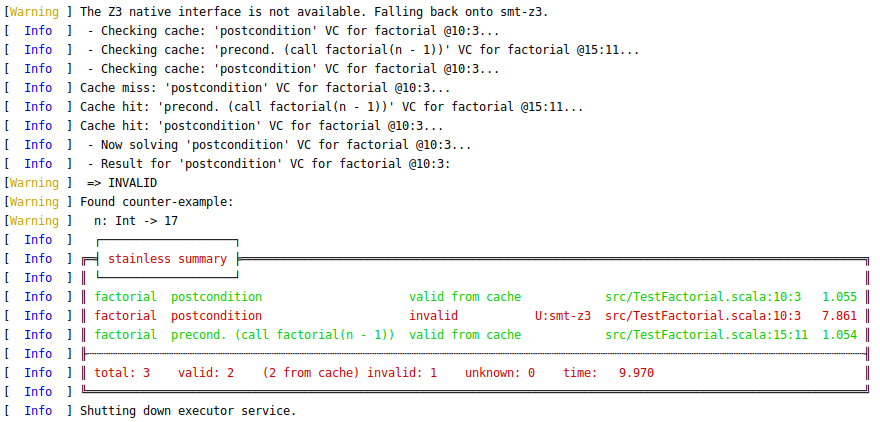
\includegraphics[width=\textwidth]{output1.png}
	\caption{Output of Stainless verification for calculating factorial of Int number}
	\label{fig:failed}
\end{figure}


\paragraph{The Pure Scala Fragment.} The Scala fragment supported by
Stainless is described in the Stainless documentation
\cite{Stainless:documentation} in the section
\href{https://epfl-lara.github.io/stainless/purescala.html}{Pure
  Scala}.

It comprises algebraic data types in the form of abstract classes,
case classes and case objects, objects for grouping classes and
functions, boolean expressions with short-circuit interpretation,
generics with invariant type parameters, default values of function
parameters, pattern matching, local and anonymous classes and more.
  
In addition to Pure Scala Stainless also supports some imperative
features, such as using a (mutable) variable in a local scope of a
function and while loops. They turn out not to be relevant for the
current work.

What will turn out to be more relevant are the following Scala
features which Stainless does not support, such as: (concrete) class
definitions, inheritance by objects, abstract type members, variance
annotations and private inner classes.

In addition, Stainless has its own library of some core data types and
functions which need to be mapped correctly to functions inside of the
SMT solver that Stainless ultimately relies on. Those data types in
general do not have all the methods of the Scala data types. For
example, the BigInt type in Scala has a methods for bitwise operations
while the BigInt type in Stainless does not.

\paragraph{Outline and Properties to Verify.} In the next section we
try to verify the property that a regular (non-coinbase) transaction
cannot generate new coins. We call it the \emph{no-inflation
  property}. Trying to verify it, we uncover and fix a bug in the
bitcoin-s library. We then find that there is too much code involved
that lies outside of the supported fragment to currently make this
verification feasible. Instead, we turn to a simpler property to
verify. The simplest possible property we can think of is the fact
that adding zero satoshis to a given amount of satoshis yields the
given amount of satoshis. We call it the \emph{addition-with-zero
  property} and we try to verify it in Section~3. Here as well we see
that a significant part of the code lies outside of the supported
fragment. However, after a series of equivalent transformations we
arrive at code that we successfully verify.


\section{The No-Inflation Property}

A crucial function for the verification of the no-inflation property
is the \texttt{checkTransaction} function, shown in
Figure~\ref{fig:checktrans}. To better understand it, we first see how
to create a transaction.

\paragraph{Creating a Transaction}

% The bitcoin-s library has a bitcoin
% transaction builder class with the following constructor:

% \begin{lstlisting}[style=scala]
% def apply(
%       destinations: Seq[TransactionOutput],
%       utxos: BitcoinTxBuilder.UTXOMap,
%       feeRate: FeeUnit,
%       changeSPK: ScriptPubKey,
%       network: BitcoinNetwork): Future[BitcoinTxBuilder] = {...}
% \end{lstlisting}

% The purpose of the return type Future is not clear to us here, since
% the constructor always returns a completed future. This might be for
% future purposes.

To create a transaction, we first need some coins -- an unspent
transaction output. We could load an actual unspent transaction output
from the bitcoin network, but we create one manually in order to see
this process. So we first create an (invalid) transaction with one
output in Figure~\ref{fig:prevtx}.

\begin{figure}
\begin{lstlisting}[style=scala]
  val privKey = ECPrivateKey.freshPrivateKey
  val creditingSPK = P2PKHScriptPubKey(pubKey = privKey.publicKey)

  val amount = Satoshis(Int64(10000))

  val utxo = TransactionOutput(currencyUnit = amount, scriptPubKey = creditingSPK)

  val prevTx = BaseTransaction(
    version = Int32.one,
    inputs = List.empty,
    outputs = List(utxo),
    lockTime = UInt32.zero
  )
\end{lstlisting}
  
  \caption{Creating a transaction output to spend}
  \label{fig:prevtx}
\end{figure}

We first create a keypair, then a lock script with its public key,
then the amount of satoshis, then a transaction output (utxo) for that
amount and locked with that script. Finally we create the actual
transaction with that output and no inputs. Of course, that is not a
valid transaction, because it creates coins out of nothing. In
particular, checkTransaction(prevTx) is false.

Now that we have a transaction output, we create a new transaction to
spend it.

First, we need some out points.  They point to outputs of previous
transactions.  We use the index zero, because the previous transaction
has only one output that becomes the first index zero.  If there were
two previous outputs, the second output would become the index 1 and
so on.
\begin{figure}
\begin{lstlisting}[style=scala]
  val outPoint = TransactionOutPoint(prevTx.txId, UInt32.zero)

  val utxoSpendingInfo = BitcoinUTXOSpendingInfo(
    outPoint = outPoint,
    output = utxo,
    signers = List(privKey),
    redeemScriptOpt = None,
    scriptWitnessOpt = None,
    hashType = HashType.sigHashAll
  )

  val utxos = List(utxoSpendingInfo)

  val destinationAmount = Satoshis(Int64(5000))

  val destinationSPK = P2PKHScriptPubKey(pubKey = ECPrivateKey.freshPrivateKey.publicKey)

  val destinations = List(
    TransactionOutput(currencyUnit = destinationAmount, scriptPubKey = destinationSPK)
  )

  val feeRate = SatoshisPerByte(Satoshis.one)

  val networkParams = RegTest // some static values for testing

  val txBuilderF: Future[BitcoinTxBuilder] = BitcoinTxBuilder(
    destinations = destinations, // where to send the money
    utxos = utxos,               // unspent transaction outputs
    feeRate = feeRate,           // fee rate per byte
    changeSPK = creditingSPK,    // where to send the change
    network = networkParams      // bitcoin network information
  )

  val txF: Future[Transaction] = txBuilderF.flatMap(_.sign)

  val tx: Transaction = Await.result(signedTxF, 1 second)
\end{lstlisting}
  \caption{Creating a transaction}
  \label{fig:tx}
\end{figure}

This utxos are the inputs of our transaction.
Second, we need destinations to spend the bitcoins to.
For the sake of convenience we create only one.
We spend 5000 satoshis to the newly created random public key.
Finally, we define the fee rate in satoshis per one byte transaction
size as well as some bitcoin network parameters.  The bitcoin network
parameters are not important, so we use some static values normally
used when testing.

Now lets build the transaction with those data.
Line one to seven creates a transaction builder which is then signed
on line ten.  We can now use our transaction object on line twelve.
For example, after calling \emph{hex} on it, we can send the returned
string to the bitcoin network.


\paragraph{Validating a Transaction}

Bitcoin-S offers a function called \emph{checkTransaction} located in the ScriptInterpreter object.

\begin{figure}
\begin{lstlisting}[style=scala]
/**
  * Checks the validity of a transaction in accordance to bitcoin core's CheckTransaction function
  * https://github.com/bitcoin/bitcoin/blob/f7a21dae5dbf71d5bc00485215e84e6f2b309d0a/src/main.cpp#L939.
  */
def checkTransaction(transaction: Transaction): Boolean = {
  val inputOutputsNotZero =
    !(transaction.inputs.isEmpty || transaction.outputs.isEmpty)
  val txNotLargerThanBlock = transaction.bytes.size < Consensus.maxBlockSize
  val outputsSpendValidAmountsOfMoney = !transaction.outputs.exists(o =>
    o.value < CurrencyUnits.zero || o.value > Consensus.maxMoney)

  val outputValues = transaction.outputs.map(_.value)
  val totalSpentByOutputs: CurrencyUnit =
    outputValues.fold(CurrencyUnits.zero)(_ + _)
  val allOutputsValidMoneyRange = validMoneyRange(totalSpentByOutputs)
  val prevOutputTxIds = transaction.inputs.map(_.previousOutput.txId)
  val noDuplicateInputs = prevOutputTxIds.distinct.size == prevOutputTxIds.size

  val isValidScriptSigForCoinbaseTx = transaction.isCoinbase match {
    case true =>
      transaction.inputs.head.scriptSignature.asmBytes.size >= 2 &&
        transaction.inputs.head.scriptSignature.asmBytes.size <= 100
    case false =>
      //since this is not a coinbase tx we cannot have any empty previous outs inside of inputs
      !transaction.inputs.exists(_.previousOutput == EmptyTransactionOutPoint)
  }
  inputOutputsNotZero && txNotLargerThanBlock && outputsSpendValidAmountsOfMoney && noDuplicateInputs &&
  allOutputsValidMoneyRange && noDuplicateInputs && isValidScriptSigForCoinbaseTx
}
\end{lstlisting}
  
  \caption{The \texttt{checkTransaction} function in the \texttt{ScriptInterpreter} object}
  \label{fig:checktrans}
\end{figure}

We can pass a transaction and it returns a Boolean indicating whether
the transaction is valid or not.  So for example when we pass the
transaction we built before the returned value would be true, because
it's a valid transaction.  It might not be accepted by the bitcoin
network but for a transaction on its own it's valid.  We can not check
context with it, because we can only pass one transaction.

There are several checks in checkTransaction.
For example, it checks if there is either no input or no output.
In this case we get false.

The relevant part for the bug we found:
\begin{lstlisting}[style=scala]
  val prevOutputTxIds = transaction.inputs.map(_.previousOutput.txId)
  val noDuplicateInputs = prevOutputTxIds.distinct.size == prevOutputTxIds.size
\end{lstlisting}

It gathers all transaction ids referenced by the out points.  When we
call \emph{distinct} on the returned list, we get a list with
duplicate removed.  If the size of the new list is the same as the
size of the old, we know that there was no duplicate transaction id,
because, as said, distinct removes the duplicates.




\paragraph{Trying Stainless on the entire project.}

\begin{itemize}
\item result sbt: no output
\item result jar: 
\end{itemize}

In order to verify a project, Stainless must be integrated into it.
We can integrate it in an sbt project adding the Stainless Plugin 
and the required resolver to pugins.sbt. 
Another option to use Stainless is to import its libraries in a program code 
and verify a program from command line using the pre-packaged Stainless JAR file 
or using the Stainless script built from source.
Trying to integrate Stainless in Bitcoin-S caused a lot of troubles,
mainly because of version conflicts.  For more details see chapter
\ref{chap:appendix_arb}.


After integrating the Stainless plugin in the Bitcoin-S sbt project, 
there were many errors because of the different sbt versions.  
Some errors are described in the section 4.2.
It takes too much time to fix them all so it should be easier to extract
the classes needed for the \texttt{checkTransaction} function.

\paragraph{Putting aside the No-Inflation Property.} Naively trying
Stainless on the entire bitcoin-s codebase results in either no output
(with sbt) or many errors (with jar). So we extract the relevant code
to only verify that. However, the extracted code has more than 1500
lines and liberally uses Scala features outside of the supported
fragment.  We tried to transform the code into the supported fragment,
but realize that a better approach is to first verify a simpler
property with less code involved and then turn back to the
no-inflation property with more experience. So we turn to the
addition-with-zero property in the next section. \todo{explain}


\paragraph{Fixing a Bug in Bitcoin-S}

We can see that there is a bug in the checkTransaction function from
before, recognized and fixed through this work.

Here is the relevant code of checkTransaction again:
\begin{lstlisting}[style=scala]
  val prevOutputTxIds = transaction.inputs.map(_.previousOutput.txId)
  val noDuplicateInputs = prevOutputTxIds.distinct.size == prevOutputTxIds.size
\end{lstlisting}

What happens if we have two TransactionOutPoints (previousOutputs) with a different index but referencing the same Transaction ID (txId)?

According to the Bitcoin protocol this is possible.  A transaction can
have multiple outputs that should be referenceable by the next
transaction.  So this is clearly a bug.

What should not be possible is a transaction referencing the same
output twice.  This bug occurred in Bitcoin Core known as
CVE-2018–17144 which was patched on September 18,
2018. \cite{cve201817144}

Here, Bitcoin-S did a bit too much and marked all transaction as
invalid, if they referenced the same transaction twice.  The fix is,
to check on TransactionOutPoint instead of TransactionOutPoint.txId,
because TransactionOutPoint contains the txId as well as the output
index it references.  So in pseudo code, we check on the tuple (tx,
index) instead of (tx).  The fixed code:
\begin{lstlisting}[style=scala]
  val prevOutputs = transaction.inputs.map(_.previousOutput)
  val noDuplicateInputs = prevOutputs.distinct.size == prevOutputs.size
\end{lstlisting}

Since TransactionOutPoint is a case class and Scala has a built in ==
for case classes there is no need to implement TransactionOutPoint.==.

This was fixed in
\href{https://github.com/bitcoin-s/bitcoin-s/pull/435}{pull request
  number 435} on GitHub at April 23, 2019, through this work along
with a unit test to prevent this bug from appearing again in the
future.


\section{The Addition-with-Zero Property}

\label{chap:verify_add}

In Bitcoin-S there is a class \texttt{Satoshis} representing an amount of bitcoins.
We look at the verification of the addition of Satoshis with zero Satoshis.
This operation should result in the same amount of Satoshis.
Let's call it the \nameref{property_2}.

Using Stainless, we see the successful verification of this property.
But the process of the verification with the tool requires many
changes in the code, so that Stainless can accept it.  We look at all
needed modifications in chapter \ref{chap:verify_add}.



After realizing that it would consume too much time to rewrite the
Bitcoin-S code and even the extracted part with checkTransaction, the
smallest unit in Bitcoin-S-Core that is worthwhile to verify was
extracted.  This could be the addition of two CurrencyUnits.  To make
it even easier, the addition of CurrencyUnits with zero.
CurrencyUnits is an abstract class in Bitcoin-S, representing
currencies like Satoshis.

\paragraph{Extracting the relevant Code}

The relevant code is in two files: \texttt{CurrencyUnits.scala} and \texttt{NumberType.scala}.

reference: code/addition/src/main/scala/addition/original

From those files we removed all code that is not needed for our
verification. For example, we removed all number types except for
Int64 (so Int32, UInt64, etc.) because we do not use them. We also
removed the superclasses Factory and NetworkElement of CurrencyUnit
and Number, respectively because the inherited members are not used by
the relevant code. Also, we removed all binary operations on Number that are not used.


  - removed extending Factory, NetworkElement and BasicArithmetic. This includes some hex/byte conversion eg fromHex, hex, bytes, fromBytes, ... Just interfaces never referenced
    \href{https://bitcoin-s.org/docs/core/core-intro\#the-basics}{description in section \#the-basics (cannot add link with hashtag)}
    \href{https://github.com/bitcoin-s/bitcoin-s/blob/master/core/src/main/scala/org/bitcoins/core/protocol/NetworkElement.scala}{NetworkElement class}
    \href{https://github.com/bitcoin-s/bitcoin-s/blob/master/core/src/main/scala/org/bitcoins/core/util/Factory.scala}{Factory class}

  - removed Bitcoins class

  - removed subtraction and multiplication, binary operations <<, >>, etc, comparision operator <=, >=, etc but not == and !=

  - removed toBigDecimal

  - removed object CurrencyUnits containing some variables to transform satoshis to btc (not used)

  The code we use for the following sections is in reduced folder.

  
Here we can see the extracted code needed for the addition of CurrencyUnits:
\lstinputlisting[style=scala]{../code/addition/src/main/scala/addition/reduced/number/NumberType.scala}
\lstinputlisting[style=scala]{../code/addition/src/main/scala/addition/reduced/currency/CurrencyUnits.scala}

The additions' signature looks like this:
\begin{lstlisting}[style=scala]
  +(c: CurrencyUnit): CurrencyUnit
\end{lstlisting}

When we run Stainless on this code (without any properties to prove),
it throws the following errors: \todo{describe errors: no support for
  abstract types, unsupported arguments for the BigInt constructor,
  unsupported inheritance for objects.}

\paragraph{Transforming the Code.}

\todo{kai todo}


\paragraph{The Specification.}

As specified, our verification must only support addition with zero.
So we restrict the parameter to be zero in the precondition.
\begin{lstlisting}[style=scala]
  require(c.satoshis == Satoshis.zero)
\end{lstlisting}

We ensure the result is the same value as \emph{this} in the postcondition.
\begin{lstlisting}[style=scala]
  ensuring(res => res.satoshis == this.satoshis)
\end{lstlisting}

We can use equals (==) directly on Satoshis, because it is a case class.

Before:
\begin{lstlisting}[style=scala]
sealed abstract class CurrencyUnit {
  def satoshis: Satoshis

  def !=(c: CurrencyUnit): Boolean = !(this == c)

  def ==(c: CurrencyUnit): Boolean = satoshis == c.satoshis

  def +(c: CurrencyUnit): CurrencyUnit = {
    Satoshis(satoshis.underlying + c.satoshis.underlying)
  }

  protected def underlying: Int64
}
\end{lstlisting}

The addition will now look like this:
\begin{lstlisting}[style=scala]
sealed abstract class CurrencyUnit {
  def satoshis: Satoshis

  def !=(c: CurrencyUnit): Boolean = !(this == c)

  def ==(c: CurrencyUnit): Boolean = satoshis == c.satoshis
  
  override def +(c: CurrencyUnit): CurrencyUnit = {
    require(c.satoshis == Satoshis.zero)
    Satoshis(satoshis.underlying + c.satoshis.underlying)
  } ensuring(res => res.satoshis == this.satoshis)

  protected def underlying: Int64
}
\end{lstlisting}

That's all we need to verify our addition.



\paragraph{Result}

Finally, everything is green and correctly verified. 
\begin{figure}
	\centering
		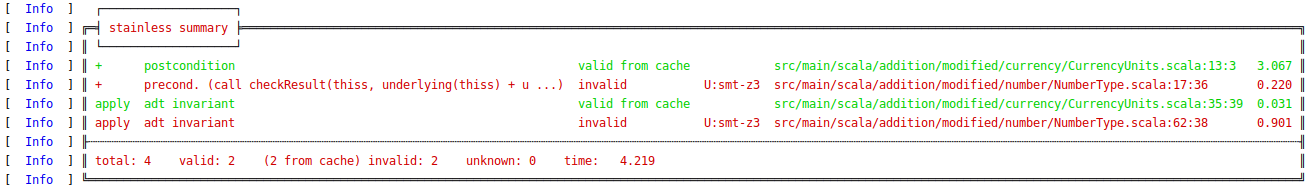
\includegraphics[width=\textwidth]{result_output}
	\caption{Output of Stainless verification for addition with 0 of Bitcoin-S-Cores CurrencyUnit}
\end{figure}

The verified code.
\lstinputlisting[style=scala]{../code/addition/src/main/scala/addition/modified/number/NumberType.scala}
\lstinputlisting[style=scala]{../code/addition/src/main/scala/addition/modified/currency/CurrencyUnits.scala}







\section{Conclusion}
\label{chap:conclusion}

Because of the limitations of the verication tool, we could only
verify a rewritten version of the original Bitcoin-S code.  So we can
not guarantee the correctness of the addition of Satoshis with zero in
Bitcoin-S.  Not all changes we made were as trivial as the replacement
of objects with case objects.  For these non-trivial changes, as seen
for example the bound check in section \ref{sec:bound_check}, we
cannot say whether they are equivalent to the original implementation
or not.

So code should be written specically with formal verication in mind,
in order to successfully verify it.  Otherwise, it needs a lot of
changes in the software because verification is mathematical and the
current software is written mostly in object-oriented style.  Software
written in the functional paradigm would be much easier to reason
about.

Thus, either Stainless must find ways to translate more of built-in
object-oriented patterns of Scala to their verification tool or
developers must invest more in functional programming.

Also, we found that trying to verify code reveals bugs as shown in
section \ref{sec:bugfix}.  Finally, our work led to some feedback to
the Stainless developers to improve the tool.

\todo{conclusions: what's future work? how to
  change bitcoin-s? how to extend stainless?}

\bibliographystyle{splncs04}
\bibliography{bibliography}


\appendix
\section{Project Setup}

In this chapter we look at the practical challenges that could occur
by using Stainless.  Since Stainless is still in development and there
is no 1.x release there might still be breaking changes and
improvements fixing problems described now.

\todo{nur über stainless-sbt-plugin reden damit man weiss wir haben es versucht}



\subsection{stainless-sbt-plugin vs JAR}

We can either use the sbt plugin or a JAR file to check code with Stainless.

Invoking the JAR on our source code Stainless will verify it.  If we
have a bigger project, this becomes really tricky, because we must
pass all files needed including the dependencies.  This is in contrast
to the sbt plugin, where we can integrate Stainless in our compilation
process.  When we call compile, Stainless verifies the code and stops
the compilation if the verification fails.

Having a static version configured in the sbt build file, every
developer has the same Stainless features available.  This should
prevent incompatibility with new or deprecated features when we use
different plugins.

So the sbt plugin has clear advantages over the JAR file since its
integrated directly.  We do not have to download it manually and find
the right version and if we bump the version we can just edit it in
the build file and every developer is on the same version again.

However, currently there are some drawbacks.  For example the sbt
plugin does not always report errors.

We use the jar for everything. 

\subsection{Integration into Bitcoin-S}

During this work, Stainless updated the sbt plugin to support sbt
1.2.8 from 0.13.17 and Scala 2.12.8 from 2.11.12.  So this section
might be out of date now.

Stainless requires and Scala recommends Java SE Development Kit 8.
Newer Java versions won't work.

To use the latest version of the sbt tool you have to build it
locally.  You can run \texttt{sbt universal:stage} in the cloned
Stainless git repository.  This generates
\emph{frontends/scalac/target/universal/stage/bin/stainless-scalac}.

Bitcoin-S-Core uses sbt 1.2.8 and Scala 2.12.8, while Stainless sbt
plugin is on sbt 0.13.17 and Scala 2.11.12.

Sbt introduced new features in the 1.x release used by Bitcoin-S.
Most of them can be written the sbt 0.13.17 way.

The bigger problem is, due to the different Scala and sbt versions,
the following error after trying to go in a sbt shell:
\begin{verbatim}
  [warn] There may be incompatibilities among your library dependencies; run 'evicted'
         to see detailed eviction warnings.
  [error] java.lang.NoClassDefFoundError: sbt/SourcePosition
  ...
  Project loading failed: (r)etry, (q)uit, (l)ast, or (i)gnore?
\end{verbatim}

Downgrading Bitcoin-S sbt version to 0.13.17 fixes the error but then
it can not load some libraries only compiled for newer versions.  So
this would take too much time to fix and changes the Bitcoin-S code
inadvertently.

The next approach is to use the stainless cli instead of sbt.  Running
stainless on all source files does not work, because dependencies are
missing.  The parameter \emph{-classpath} can resolve it but the value
of this parameter must be the paths to all the dependencies separated
by a ':'.  Finally, \emph{core} depends on \emph{secp256k1jni},
another package of Bitcoin-S written in Java.  So this needs to be in
the source files to.

The final command looks like this in \emph{core} folder of Bitcoin-S:
\begin{lstlisting}[language=bash]
  $ stainless
    -classpath ".:$(find ~/.ivy2/ -type f -name *.jar | tr '\n' ':')"
    $(find . -type f -name *.scala | tr '\n' ' ')
    $(find ../secp256k1jni -type f -name *.java | tr '\n' ' ')
\end{lstlisting}

\emph{.ivy2} is the dependency cache of sbt.  The \emph{tr} replaces
the first char with the second so a newline with either ':' or ' '.

With this command, Stainless throws the next error:
\begin{verbatim}
  [Internal] Error: object scala.reflect.macros.internal.macroImpl in compiler mirror
             not found.. Trace:
  [Internal] - scala.reflect.internal.MissingRequirementError$.signal
             (MissingRequirementError.scala:17)
  ...
  [Internal] object scala.reflect.macros.internal.macroImpl in compiler mirror not found.
  [Internal] Please inform the authors of Inox about this message
\end{verbatim}

So we can not know how many errors will face us.  Let's go another
way, because the errors may take too much time and it might lead to a
next error.  We extract the code needed to verify a transaction mainly
the class Transaction and ScriptInterpreter with many other classes
they're depending on.

After this extraction Stainless was successfully integrated with both
sbt and JAR.

Running \texttt{sbt compile} in the project with Stainless ended
without error.  But it also ended with no output.  So we are not able
to change the code so Stainless would accept it since we do not know
what to change.

So the sbt plugin does not always complain where the JAR file did.
The open
\href{https://github.com/epfl-lara/stainless/issues/484}{issue 484 on
  GitHub} might describe exactly this error.

Now we can finally run Stainless on our code.  But this leads us to
the next findings.  We must rewrite most of the code, as described in
the previous chapters.


\begin{itemize}
\item clone our repo
\item jar vs sbt, you can use both
\item contains a stainless jar
\item call the script blahblah
\end{itemize}


\section{NumberType.scala}
\lstinputlisting[style=scala]{../code/addition/src/main/scala/addition/reduced/number/NumberType.scala}

\section{CurrencyUnits.scala}
\lstinputlisting[style=scala]{../code/addition/src/main/scala/addition/reduced/currency/CurrencyUnits.scala}


\section{Code Transformations} 

Here we see in detail how to transform the bitcoin-s code into the
Scala fragment supported by Stainless. All subsections start with the
Stainless error message(s) and finally a description of the changes we
make to the code.

We claim that all transformations are equivalent in the sense that if
the addition-with-zero property holds for the transformed code, then
it also holds for the code before the transformation.


\subsection{Inheriting Objects}


\begin{lstlisting}[style=stainless]
[ Error  ] number/NumberType.scala:65:1: Objects cannot extend classes or implement traits, use a case object instead
          object Int64 extends BaseNumbers[Int64] {
          ^^^^^^^^^^^^^^^^^^^^^^^^^^^^^^^^^^^^^^^^^...
[ Error  ] currency/CurrencyUnits.scala:33:1: Objects cannot extend classes or implement traits, use a case object instead
          object Satoshis extends BaseNumbers[Satoshis] {
          ^^^^^^^^^^^^^^^^^^^^^^^^^^^^^^^^^^^^^^^^^^^^^^^...
\end{lstlisting}

Here, we can just turn the objects into case objects by literally just
changing the word \texttt{object} into \texttt{case object} on lines
65 and 33 in the two respective files.

That transformation is equivalent. Case objects have some additional
properties (in particular, being serializable) and they inherit from
\texttt{Product} instead of \texttt{AnyRef}, but none of our code
depends on any of that.


\subsection{Abstract Type Members}


\begin{lstlisting}[style=stainless]
[ Error  ] currency/CurrencyUnits.scala:6:3: Stainless doesn't support abstract type members
            type A
            ^^^^^^
\end{lstlisting}

Note that we can not simply replace the unsupported abstract type
member by a (supported) type parameter. The problem is that the
CurrencyUnit class uses one of its implementing classes: Satoshis.

Satoshis would have to instantiate a potential type parameter with
type Int64, so it would extend CurrencyUnit[Int64]. But that is too
specific, because the return type of the \texttt{+}-method would then then be
CurrencyUnit[Int64] not CurrencyUnit[A].

Since we only want to verify the addition of satoshis, and the
Satoshis class overrides A with Int64 anyway, we just remove the
abstract type and set it to Int64.

We remove line 6 and line 22 from CurrencyUnits.scala (to maintain
line numbers we actually replace them with empty lines for now) and in
line 18 we replace A by Int64.


\subsection{Non-Literal BigInt Constructor Argument}


\begin{lstlisting}[style=stainless]
[ Error  ] currency/CurrencyUnits.scala:26:33: Only literal arguments are allowed for BigInt.
            def toBigInt: BigInt = BigInt(toLong)
                                          ^^^^^^
\end{lstlisting}

As described before, the types in the Stainless library are more
restricted than their Scala library counterparts. In particular, the
Stainless BigInt constructor is restricted to literal arguments.


After:
\begin{lstlisting}[style=scala]
sealed abstract class Satoshis extends CurrencyUnit {
  override def satoshis: Satoshis = this

  def toBigInt: BigInt = underlying.toBigInt

  def toLong: Long = underlying.toLong

  def ==(satoshis: Satoshis): Boolean = underlying == satoshis.underlying
}
\end{lstlisting}


Here we can simply use toBigInt on the field \texttt{underlying}
directly.  So, instead of converting the underlying to Long and back
to BigInt we convert underlying directly to BigInt.

We replace line 26 by
\begin{lstlisting}[style=scala]
def toBigInt: BigInt = underlying.toBigint
\end{lstlisting}

This is an equivalent transformation: the only thing that might go
wrong in the detour via \texttt{Long} is that the BigInt underlying
Int64 in turn underlying Satoshis does not fit into a Long. However,
the only constructor of Int64 ensures exactly that.

\subsection{Self-Reference in Type Parameter Bound}

\begin{lstlisting}[style=stainless]
[ Error  ] number/NumberType.scala:8:30: Unknown type parameter type T
          sealed abstract class Number[T <: Number[T]] {
                                        ^^^^^^^^^^^^^^
\end{lstlisting}

Stainless does not currently support a class with a type parameter
with a type boundary that contains the type parameter itself. We opened an
issue \cite{Stainless:issue519} on the Stainless repository and the
Stainless developers have targeted Stainless version 0.4 to support
such self-referential type boundaries.

For now, since our code only uses Number with type parameter T
instantiated to Int64, we just remove the type parameter and replace
it by Int64. We respectively replace lines 8, 44 and 49 by
\begin{lstlisting}[style=scala]
sealed abstract class Number {
\end{lstlisting}

\begin{lstlisting}[style=scala]
sealed abstract class SignedNumber extends Number
\end{lstlisting}

\begin{lstlisting}[style=scala]
sealed abstract class Int64 extends SignedNumber {
\end{lstlisting}

and replace T by Int64 in lines 25-27.


\subsection{Missing Member \texttt{bigInteger} in BigInt}


\begin{lstlisting}[style=stainless]
[ Error  ] number/NumberType.scala:14:22: Unknown call to bigInteger on Number.this.toBigInt (BigInt) with arguments List() of type List()
            def toLong: Long = toBigInt.bigInteger.longValueExact()
                              ^^^^^^^^^^^^^^^^^^^
\end{lstlisting}
\todo{stainless error emssage missing}

The Scala class BigInt is essentially a wrapper around
java.math.BigInteger. BigInt has a member bigInteger which is the
underlying instance of the Java class. The Java class has a method
longValueExact which returns a long only if the BigInteger fits into a
long, otherwise throws exception. Stainless does not support Java
classes and in particular its BigInt has no member bigInteger.

However, our code never calls toLong anymore, so we just remove it. We
replace line 14 in NumberType.scala and line 28 in CurrencyUnits.scala
by an empty line.


\subsection{Type Member}

\begin{lstlisting}[style=stainless]
[Warning ] number/NumberType.scala:9:3: Could not extract tree in class: type A = BigInt (class scala.reflect.internal.Trees$TypeDef)
              type A = BigInt
              ^^^^^^^^^^^^^^^
\end{lstlisting}

Our version of Stainless does not support type members. We just
replace all occurrence of A with BigInt, since A is never overwritten
in an implementing class.

We remove line 9 in NumberType.scala and replace A by BigInt in lines
12, 25, 33 and 50.

In the mean time Stainless has implemented support for type member
\cite{Stainless:pull470}.  Since version 0.2 verification should
succeed without this change.



\subsection{Missing Bitwise-And Method on BigInt}

\begin{lstlisting}[style=stainless]
[ Error  ] number/NumberType.scala:34:14: Unknown call to & on result (BigInt) with arguments List(Number.this.andMask) of type List(BigInt)
              require((result & andMask) == result,
                      ^^^^^^^^^^^^^^^^
\end{lstlisting}

Contrary to Scala BigInt, the Stainless BigInt class does not support
bitwise operations, in particular not the \&-method for bitwise and.

The bitwise and with the andMask on line 34 is a bounds check.  It
checks if the result parameter is in range of the specified type,
which in our case is the hard coded Int64.

So, we replace the \& mask with a check whether the result
is in range of Long.MinValue and Long.MaxValue, because Int64 has the
same 64-bit range as Long.  

We replace lines 34-35 by the following, squeezed into two lines to
preserve line numbers. Note that the BigInt constructor requires a
literal:

\begin{lstlisting}[style=scala]
require(result <= BigInt("9223372036854775807")  
  && result >= BigInt("-9223372036854775808"),
      "Result was out of bounds, got: " + result)
\end{lstlisting}


\todo{kai here we do not know if it changes semantic. ramon: oh, we don't?}



\subsection{Inner Class in Case Object}

\begin{lstlisting}[style=stainless]
[Warning ] number/NumberType.scala:66:3: Could not extract tree in class: case private class Int64Impl extends Int64 with Product with Serializable {
...
[Warning ] } (class scala.reflect.internal.Trees$ClassDef)
              private case class Int64Impl(underlying: BigInt) extends Int64 {
              ^^^^^^^^^^^^^^^^^^^^^^^^^^^^^^^^^^^^^^^^^^^^^^^^^^^^^^^^^^^^^^^^...
...
[Warning ] currency/CurrencyUnits.scala:42:3: Could not extract tree in class: case private class SatoshisImpl extends Satoshis with Product with Serializable {
...
[Warning ] } (class scala.reflect.internal.Trees$ClassDef)
              private case class SatoshisImpl(underlying: Int64) extends Satoshis
              ^^^^^^^^^^^^^^^^^^^^^^^^^^^^^^^^^^^^^^^^^^^^^^^^^^^^^^^^^^^^^^^^^^^
\end{lstlisting}

Stainless does not support inner classes in a case object. Bitcoin-s
uses this a lot to separate the class \todo{ramon: i don't understand} from its implementation.

This is easy to fix. We just move the inner classes out of the case objects. They do
not interfere with any other code.

We remove lines 66-71 in NumberType.scala and insert them at the end of the file.
We remove line 42 in CurrencyUnits.scala and insert it at the end of the file.


\subsection{Message Parameter in Require}

\begin{lstlisting}[style=stainless]
[Warning ] number/NumberType.scala:67:3: Could not extract tree in class: scala.this.Predef.require(Int64Impl.this.underlying.>=(math.this.BigInt.long2bigInt(-9223372036854775808L)), "Number was too small for a int64, got: ".+(Int64Impl.this.underlying)) (class scala.reflect.internal.Trees$Apply)
          require(underlying >= -9223372036854775808L,
          ^^^^^^^^^^^^^^^^^^^^^^^^^^^^^^^^^^^^^^^^^^^^...
[Warning ] number/NumberType.scala:69:3: Could not extract tree in class: scala.this.Predef.require(Int64Impl.this.underlying.<=(math.this.BigInt.long2bigInt(9223372036854775807L)), "Number was too big for a int64, got: ".+(Int64Impl.this.underlying)) (class scala.reflect.internal.Trees$Apply)
          require(underlying <= 9223372036854775807L,
          ^^^^^^^^^^^^^^^^^^^^^^^^^^^^^^^^^^^^^^^^^^^...
[ Error  ] checkResult$0 depends on missing dependencies: require$1.
\end{lstlisting}

Here the require(condition, message) is used as an assertion: if the
condition is false the fail with message.  Stainless does not support
the message parameter of require.  For the verification we can simply
remove that parameter.



\subsection{Missing Implicit Long to BigInt Conversion}

\begin{lstlisting}[style=stainless]
[ Error  ] inv$4 depends on missing dependencies: long2bigInt$0.
\end{lstlisting}

This error message does not specify a line number and it is not clear
what ``inv'' is. However, the Scala BigInt has implict conversions
from Long and they are missing in the Stainless BigInt.



We replace the two require clauses at lines 67 and following in NumberType.scala

\begin{lstlisting}[style=scala]
  require(underlying >= -9223372036854775808L)
  require(underlying <= 9223372036854775807L)
\end{lstlisting}

by:
\begin{lstlisting}[style=scala]
  require(underlying >= BigInt(-9223372036854775808L))
  require(underlying <= BigInt(9223372036854775807L))
\end{lstlisting}

We also replace lines 76 and 77
\begin{lstlisting}[style=scala]
  lazy val min = Int64(-9223372036854775808L)
  lazy val max = Int64(9223372036854775807L)
\end{lstlisting}

by:
\begin{lstlisting}[style=scala]
  lazy val min = Int64(BigInt(-9223372036854775808L))
  lazy val max = Int64(BigInt(9223372036854775807L))
}
\end{lstlisting}


\subsection{Missing BigInt Constructor with Long Argument}

\begin{lstlisting}[style=stainless]
[ Error  ] apply$14 depends on missing dependencies: BigInt$0, apply$15.
\end{lstlisting}

Here again, the Scala BigInt has a constructor with a Long argument
which is missing in the Stainless BigInt.

We simply replace the Long values in a BigInt constructor call with a string
literal.

The lines from the previous transformation respectively change into
the following:

\begin{lstlisting}[style=scala]
  require(underlying >= BigInt("-9223372036854775808"))
  require(underlying <= BigInt("9223372036854775807"))
\end{lstlisting}

and

\begin{lstlisting}[style=scala]
  lazy val min = Int64(BigInt("-9223372036854775808"))
  lazy val max = Int64(BigInt("9223372036854775807"))
}
\end{lstlisting}



\end{document}
